\documentclass[reprint,english,notitlepage]{revtex4-1}  % defines the basic parameters of the document

% if you want a single-column, remove reprint

% allows special characters (including æøå)
\usepackage[utf8]{inputenc}
\usepackage[english]{babel}
\usepackage{comment}

%% note that you may need to download some of these packages manually, it depends on your setup.
%% I recommend downloading TeXMaker, because it includes a large library of the most common packages.

\usepackage{physics,amssymb}  % mathematical symbols (physics imports amsmath)
\usepackage{graphicx}         % include graphics such as plots
\usepackage{xcolor}           % set colors
\usepackage{hyperref}         % automagic cross-referencing (this is GODLIKE)
\usepackage{tikz}             % draw figures manually
\usepackage{listings}         % display code
\usepackage{subfigure}        % imports a lot of cool and useful figure commands

% defines the color of hyperref objects
% Blending two colors:  blue!80!black  =  80% blue and 20% black
\hypersetup{ % this is just my personal choice, feel free to change things
    colorlinks,
    linkcolor={red!50!black},
    citecolor={blue!50!black},
    urlcolor={blue!80!black}}

%% Defines the style of the programming listing
%% This is actually my personal template, go ahead and change stuff if you want
\lstset{ %
	inputpath=,
	backgroundcolor=\color{white!88!black},
	basicstyle={\ttfamily\scriptsize},
	commentstyle=\color{magenta},
	language=Python,
	morekeywords={True,False},
	tabsize=4,
	stringstyle=\color{green!55!black},
	frame=single,
	keywordstyle=\color{blue},
	showstringspaces=false,
	columns=fullflexible,
	keepspaces=true}


%% USEFUL LINKS:
%%
%%   UiO LaTeX guides:        https://www.mn.uio.no/ifi/tjenester/it/hjelp/latex/ 
%%   mathematics:             https://en.wikibooks.org/wiki/LaTeX/Mathematics

%%   PHYSICS !                https://mirror.hmc.edu/ctan/macros/latex/contrib/physics/physics.pdf

%%   the basics of Tikz:       https://en.wikibooks.org/wiki/LaTeX/PGF/TikZ
%%   all the colors!:          https://en.wikibooks.org/wiki/LaTeX/Colors
%%   how to draw tables:       https://en.wikibooks.org/wiki/LaTeX/Tables
%%   code listing styles:      https://en.wikibooks.org/wiki/LaTeX/Source_Code_Listings
%%   \includegraphics          https://en.wikibooks.org/wiki/LaTeX/Importing_Graphics
%%   learn more about figures  https://en.wikibooks.org/wiki/LaTeX/Floats,_Figures_and_Captions
%%   automagic bibliography:   https://en.wikibooks.org/wiki/LaTeX/Bibliography_Management  (this one is kinda difficult the first time)
%%   REVTeX Guide:             http://www.physics.csbsju.edu/370/papers/Journal_Style_Manuals/auguide4-1.pdf
%%
%%   (this document is of class "revtex4-1", the REVTeX Guide explains how the class works)


%% CREATING THE .pdf FILE USING LINUX IN THE TERMINAL
%% 
%% [terminal]$ pdflatex template.tex
%%
%% Run the command twice, always.
%% If you want to use \footnote, you need to run these commands (IN THIS SPECIFIC ORDER)
%% 
%% [terminal]$ pdflatex template.tex
%% [terminal]$ bibtex template
%% [terminal]$ pdflatex template.tex
%% [terminal]$ pdflatex template.tex
%%
%% Don't ask me why, I don't know.

\begin{document}
\title{Temperfect mug}   % self-explanatory
\author{Tor-Andreas Bjone}               % self-explanatory
\date{\today}                             % self-explanatory
\noaffiliation                            % ignore this
\begin{abstract}                          % marks the beginning of the abstract
We looked at the difference between a regular thermos cup (Bodum) and the Temperfect mug by measuring the temperature as a function of time. We found that the temperature was higher in the Temperfect mug because it reduced the temperature difference $\nabla T$ between the liquid in the mug and the room at the beginning by absorbing heat from the liquid and preforming a phase transition between solid and liquid itself. This gave it latent heat that it could later give back to the liquid in the mug by going back to a solid. The codes can be found on my GitHub: \url{https://github.com/Trrn13P/FYS2160/tree/master/Oblig_1}
                % the body of the abstract
\end{abstract}                            % marks the end of the abstract
\maketitle                                % creates the title, author, date & abstract


% the fundamental components of scientific reports:
\section{Introduction}
In this experiment we have looked at the temperature of a liquid in two thermos cups. The Bodum cup and the temperfect cup. We pour almost boiling liquid into the cups and measure the temperature as a function of time. We did not put the lids on the cups since it would be to much of a hassle to drill two holes in the top. 

The Bodum cup is just a regular thermos cup. The temperfect cup has a material that melts and thereby removing a lot of heat from the liquid in the cup, and thereafter giving that heat back by going back to a solid. This energy given up during a phase transition is called latent heat. 

We will look at the temperature graphs to see if the temperfect mug preforms as advertised and discuss if it can be modelled using an Einstein crystal. You can read about the Einstein crystal in appendix 2(\ref{appendix_2}).






\section{Theory}
The multiplicity of an Einstein crystal is given by 
\begin{equation}
 \Omega(N,q)\approx \frac{(q+N)!}{q!N!},
 \label{eq:omega}
 \end{equation}
 where $q$ is the number of energy units $\epsilon=hf$, where $f$ is the frequency and $h$ is Planck's constant, and $N$ is the number of particles in the crystal. We use this to find the entropy
  \begin{equation}
  S=k\ln\Omega,
   \label{eq:entropy}
 \end{equation}
  where $k$ is Boltzmann's constant. We have that the internal energy of the crystal is 
  \begin{equation}
  U=q\epsilon+\frac{N}{2}\epsilon,
     \label{eq:energy}
 \end{equation}
  if we include the ground-states. This of course gives us that 
  \begin{equation}
   dU=\epsilon dq,
      \label{eq:delta_energy}
 \end{equation}
  since we vary $q$. 
  
  The thermodynamic identity says that 
  \begin{equation}
  dU=TdS-PdV+\mu dN,
     \label{eq:delta_energy_2}
 \end{equation}
  where $\mu$ is the chemical potential, $P$ is the pressure and $V$ is the volume. We assume that the volume, pressure and number of particles stay constant. We then get that
  \begin{equation}
  T= \frac{dU}{dS}=\epsilon\frac{dq}{dS}\Leftrightarrow \frac{T}{\epsilon}=\frac{dq}{dS}.
     \label{eq:temperature}
 \end{equation}
  Numerically we find this as
  \begin{equation}
  \tilde{T_i} =\frac{T_i}{\epsilon}=\frac{q_i-q_{i-1}}{S_i-S_{i-1}}.
     \label{eq:temperature_numerically}
 \end{equation}

We have that the heat capacity 
\begin{equation}
C_V=\frac{dU}{dT}=\epsilon\frac{dq}{dT}=\frac{dq}{dT/\epsilon}=\frac{dq}{d\tilde{T}}.
   \label{eq:heat_capacity}
 \end{equation}
We find this numerically as 
\begin{equation}
 C_{V,i}=\frac{q_{i}-q_{i-1}}{\tilde{T}_i-\tilde{T}_{i-1}}.
    \label{eq:heat_capacity_numerically}
 \end{equation}

\section{Method}

\begin{figure}
\centering
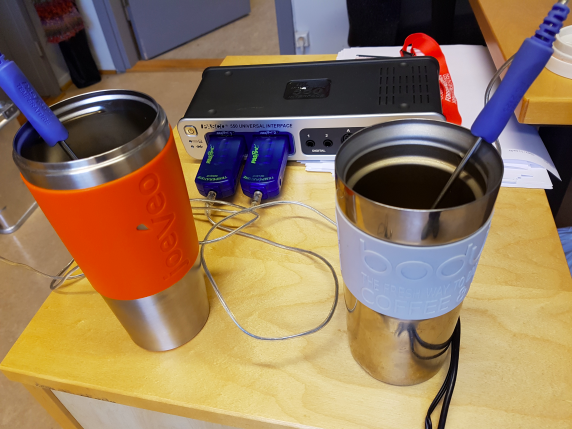
\includegraphics[width=8cm]{../figures/termos_bilder.png}
\caption{Probes measuring temperature. Temperfect mug on the left and Bodum mug on the right.}
\label{fig:termos_bilder}
\end{figure}

We insert temperature probes into the Bodum and Temperfect mug as shown in figure (\ref{fig:termos_bilder}). We start taking the temperature. Then we pour hot water into the cups. 

We use eq.\ref{eq:temperature_numerically} to find the temperature numerically as a function of the number of energy units in the crystal. And when we have the temperature we use eq.\ref{eq:heat_capacity_numerically} to find the heat capacity. Both expressions will simplify a bit since $dq=1$.

\section{Results}

\begin{figure}
\centering
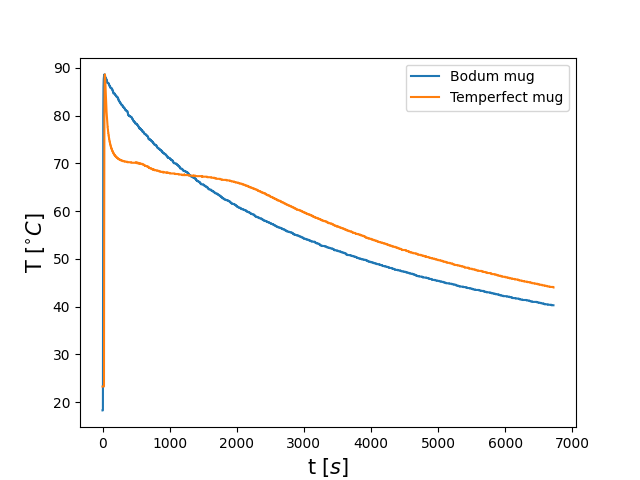
\includegraphics[width=8cm]{../figures/mugs.png}
\caption{Temperature against time for the two mugs.}
\label{fig:mugs}
\end{figure}

\begin{figure}
\centering
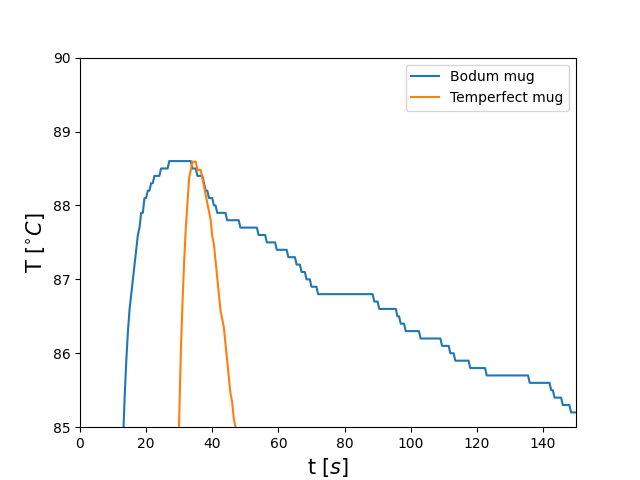
\includegraphics[width=8cm]{../figures/mugs_2.png}
\caption{Closeup of the starting points where the hot water is poured in.}
\label{fig:mugs_2}
\end{figure}


In figure (\ref{fig:mugs}) we can see the temperature of the Temperfect mug and the Bodum mug plotted against the time. Since the water was not poured at the same temperature this has been adjusted in the plot as seen in figure (\ref{fig:mugs_2}). 

We can see from figure (\ref{fig:mugs}) that the Temperfect mug absorbs a lot of heat very quickly. This is because it goes trough a phase change, from solid to liquid. It then slowly goes back to solid again and gives heat back to the liquid in the mug. That makes it so that the temperature of the liquid drops more slowly. When all of the material in the mug is solid, the liquid will drop in temperature as if it was a regular mug, like the Bodum.

The reason this is beneficial is that the heat flux is related to the $\nabla T$, so by reducing the temperature quickly, and storing it as latent heat, you can re-introduce it to the liquid later, at a lower temperature and therefore reduce the heat flux.

The assumptions in such a system that $V,P,N=const$ is reasonable. The volume change will be minimal, the number of particles will be about the same since we are good under $100^{\circ}C$ and the pressure is said to be constant. It will probably go as $\Delta P=C\Delta T$, where $C$ is a constant. I assume this constant is small. This happens between ca. $0-2000$s. 






\section{Conclusion}

We can use this to model how $q$ changes in the mug, changes the temperature of the mug material. But the Einstein solid is not valid for liquids. The Temperfect mug has a material that will melt when you put hot liquid in the mug and therefore the Einstein model is not valid at that point. After a period of time the mug material will go back into solid and here the Einstein model might be valid. As energy units is transferred from the mug material to the liquid in the mug. 



\newpage
%% if you want to include an appendix, this is how you do it
\appendix
\section*{Appendix I.}

In figure (\ref{fig:mugs}) we can see the temperature of the Temperfect mug and the Bodum mug plotted against the time. Since the water was not poured at the same temperature this has been adjusted in the plot as seen in figure (\ref{fig:mugs_2}). 

We can see from figure (\ref{fig:mugs}) that the Temperfect mug absorbs a lot of heat very quickly. This is because it goes trough a phase change, from solid to liquid. It then slowly goes back to solid again and gives heat back to the liquid in the mug. That makes it so that the temperature of the liquid drops more slowly. When all of the material in the mug is solid, the liquid will drop in temperature as if it was a regular mug, like the Bodum. 

The reason this is beneficial is that the heat flux is related to the $\nabla T$, so by reducing the temperature quickly, and storing it as latent heat, you can re-introduce it to the liquid later, at a lower temperature and therefore reduce the heat flux.






Assume constant pressure $P$ and volume $V$. This means that the work $W=0$, so that the change in internal energy $dU=dQ$. We also assume a constant number of particles $N$. In this condition we can use the definition of temperature(given by the total differential of the entropy $S$), so that the temperature $T$ is given by

$$T^{-1}=(\frac{\partial S}{\partial U})_{N,V},$$
Since we only have that $S$ is a function of $T$ we get that 
$$
T^{-1}=\frac{d S}{d U}= \frac{dS}{dQ} =\frac{d S}{dT}\frac{d T}{d Q}.
$$

$$ T^{-1}\frac{dQ}{dT}=\frac{dS}{dT}.$$

Under constant volume the heat capacity $C_V=(\partial U/\partial T)_{V,N}$, that becomes $C_V=(dQ/dT)$ in our case. We then get that 
\begin{equation}\label{}
\frac{dS}{dT}=\frac{C_V}{T}.
\end{equation}


In figure (\ref{fig:dSdT_mot_T}) we see the slope of the entropy $dS/dT$ against the temperature $T$, calculated by this method in H2O. The heat capacity of H2O is listed in \ref{table:h2o}. We use this to calculate the entropy. In figure (\ref{fig:S_mot_T}) we see the entropy against the temperature.

\begin{table}[h]  % h = "here"  , h! = here!
\caption{Table of the heat capacity $C$ of H2O in $kJ/kgK$.}\label{table:h2o}
\begin{tabular}{|c|c|} % note that & separates columns while \\ separates the rows
\hline                    % creates a horizontal line (try removing it)
Solid & $2.108$  \\
\hline
Liquid & $4.184$ \\
\hline
Gas & $1.996$ \\
\hline
\end{tabular}
\end{table}


\begin{figure}
\centering
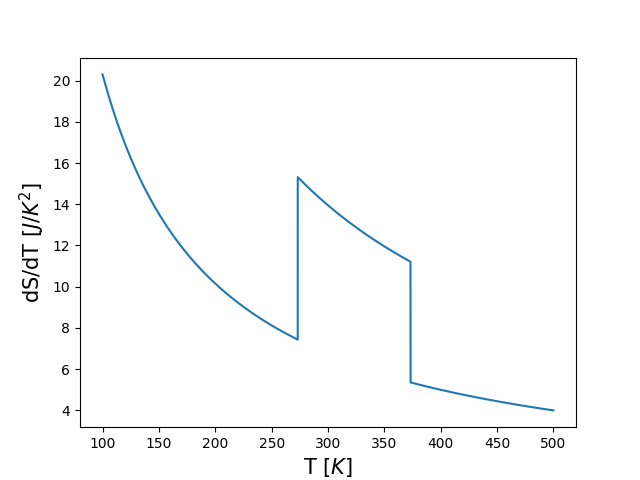
\includegraphics[width=8cm]{../figures/dSdT_mot_T.png}
\caption{Figure of the slope of entropy $dS/dT$ against the temperature $T$.}
\label{fig:dSdT_mot_T}
\end{figure}

\begin{figure}
\centering
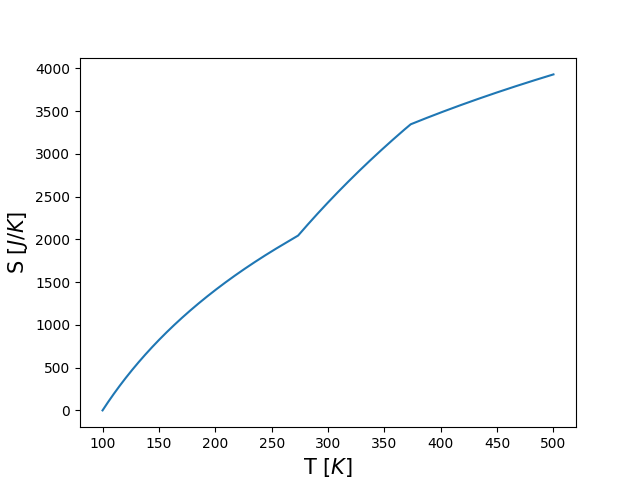
\includegraphics[width=8cm]{../figures/S_mot_T.png}
\caption{Figure of the entropy $S$ against the temperature $T$.}
\label{fig:S_mot_T}
\end{figure}



The feature of the graph that is relevant is the part where the phase changes are happening. That is from ca. $0$s to $2000$s.
\appendix
\label{appendix_2}
\section*{Appendix II.}

\subsection*{A.}
The multiplicity of an Einstein crystal is given by 
$$ \Omega(N,q)\approx \frac{(q+N)!}{q!N!},$$
 where $q$ is the number of energy units $\epsilon=hf$, where $f$ is the frequency and $h$ is Planck's constant, and $N$ is the number of particles in the crystal. We use this to find the entropy
  $$S=k\ln\Omega,$$ 
  where $k$ is Boltzmann's constant. We have that the internal energy of the crystal is 
  $$U=q\epsilon+\frac{N}{2}\epsilon,$$
  if we include the ground-states. This of course gives us that 
  $$ dU=\epsilon dq,$$
  since we vary $q$. 
  
  The thermodynamic identity says that 
  $$ dU=TdS-PdV+\mu dN,$$
  where $\mu$ is the chemical potential, $P$ is the pressure and $V$ is the volume. We assume that the volume, pressure and number of particles stay constant. We then get that
  $$T= \frac{dU}{dS}=\epsilon\frac{dq}{dS}\Leftrightarrow \frac{T}{\epsilon}=\frac{dq}{dS}.$$
  Numerically we find this as
  $$\tilde{T_i} =\frac{T_i}{\epsilon}=\frac{q_i-q_{i-1}}{S_i-S_{i-1}}.$$

We have that the heat capacity 
$$C_V=\frac{dU}{dT}=\epsilon\frac{dq}{dT}=\frac{dq}{dT/\epsilon}=\frac{dq}{d\tilde{T}}.$$
We find this numerically as 
$$ C_{V,i}=\frac{q_{i}-q_{i-1}}{\tilde{T}_i-\tilde{T}_{i-1}}.$$

\begin{figure}
\centering
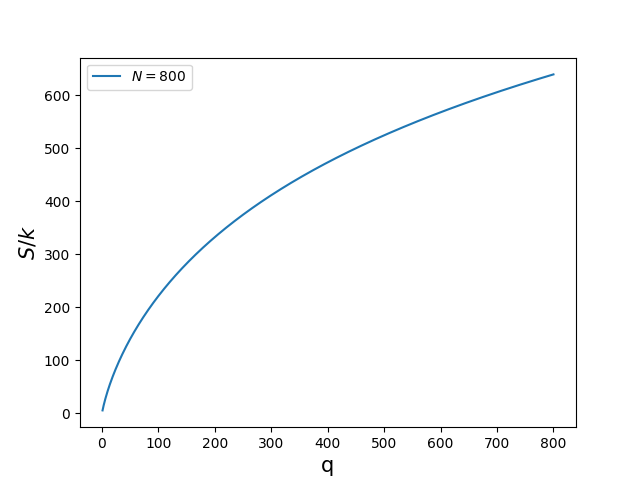
\includegraphics[width=8cm]{../figures/S_mot_q.png}
\caption{Figure of numerically calculated entropy $S/k$ against the number of energy units $q$.}
\label{fig:S_mot_q}
\end{figure}
  
\begin{figure}
\centering
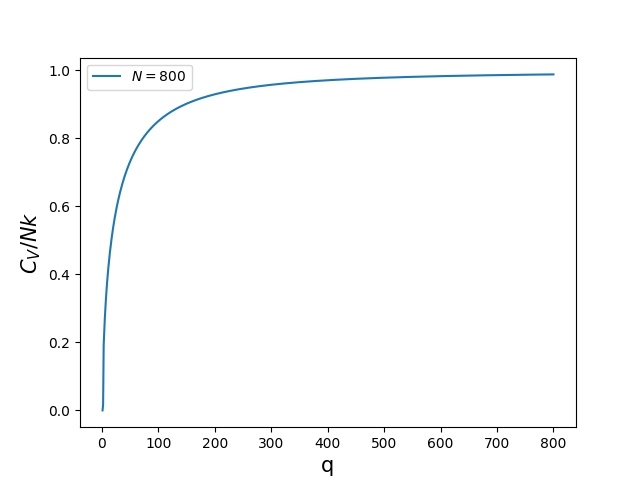
\includegraphics[width=8cm]{../figures/C_mot_q.png}
\caption{Figure of numerically calculated heat capacity $C_V$ against the number of energy units $q$.}
\label{fig:C_mot_q}
\end{figure}

We see $S/k$ as a function of $q$ in figure (\ref{fig:S_mot_q}) and $\frac{C_V}{Nk}$ as a function of $q$ in figure (\ref{fig:C_mot_q}).

\subsection*{B.}

We have that the multiplicity of an Einstein solid is $$\Omega(N,q)=\frac{(q+N-1)!}{q!(N-1)!},$$
where $N$ is the number of particles and $q$ is the number of energy units $\hbar f$. If we use $N>>1$, we can see that $$ \Omega(N,q)\approx \frac{(q+N)!}{q!N!}.$$

If also have $q>>1$ we can Stirling approximate this expression. That means that the temperature is $T>0K$. This gives us that
$$ \Omega = \frac{(q+N)!}{q!N!}\approx\frac{(q+N)^{q+N} e^{-(q+N)}}{q^q e^{-q} N^N e^{-N}}=(\frac{q+N}{q})^q(\frac{q+N}{N})^N$$ 
\\~\\
From the lectures we have that the multiplicity for the low temperature limit is $$\Omega_{low\ T}(q,N)\approx (\frac{Ne}{q})^q.$$
And the high temperature limit is $$ \Omega_{high\ T}\approx (\frac{qe}{N})^N.$$

\begin{figure}
\centering
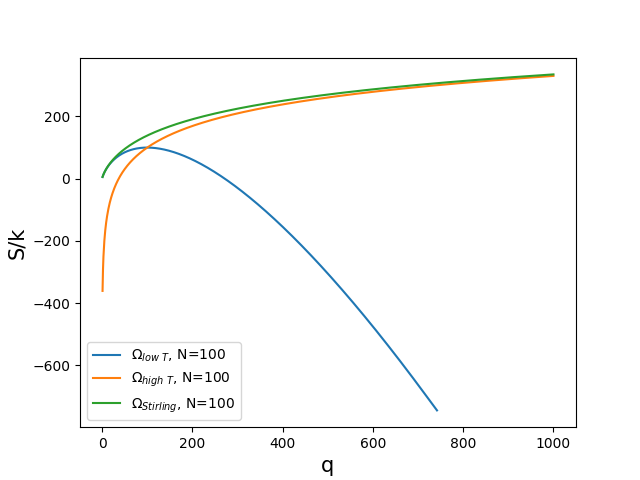
\includegraphics[width=8cm]{../figures/omegas.png}
\caption{Figure of the low temperature approximation of the multiplicity $\Omega_{low\ T}$ vs. the high temperature approximation $\Omega_{high\ T}$ vs. the Stirling approximation $\Omega_{Stirling}$ against the number of energy units $q$.}
\label{fig:omegas}
\end{figure}

We see the comparison of the different $\Omega$'s against each other in figure (\ref{fig:omegas}). From the figure we see that the low temperature approximation fits the Stirling approximation at low $q$ and the high temperature approximation at high $q$.

~\\
We had that $$dS=\frac{1}{U/Nk}dU=\frac{Nk}{U}dU=\frac{2Nk}{2q+N}dq.$$

This gives us that the entropy is $$S(U,N)=Nk\int_{U_0}^U \frac{1}{U}dU=Nk ln\frac{U}{U_0},$$

where $U_0=(1/2)N\epsilon$ is the ground state energy.
~\\

 We have that the temperature $$T(U,N)=(\frac{\partial S}{\partial U})^{-1}=(Nk\frac{1}{U})^{-1}=\frac{U}{Nk}.$$
 ~\\
 And that the heat capacity $$C_V(T,N)=\frac{dU}{dT}=\frac{d}{dT}(NkT)=Nk.$$

The specific heat capacity per. mole is $$ c=\frac{C}{n}=\frac{Nk}{n},$$
where $n=N/N_A$ is the number of moles and $N_A$ is Avogadro's number. We then get that 
$$ c=\frac{Nk}{N/N_A}=N_Ak=R,$$
where $R$ is the universal gas constant.

\subsection*{C.}
We see from figure (\ref{fig:C_mot_q}) that $C_V/Nk$ goes to one. This means that our analytical and numerical results corresponds more and more as $q$ gets higher. And in (\ref{fig:comparrison}) we see the heat capacity for different $\epsilon$. We see that this does not go to $3R$ as they should and concludes that there is something wrong in the code. We can therefore not use this for a comparison to find the $\epsilon$ of a real material.

\begin{figure}
\centering
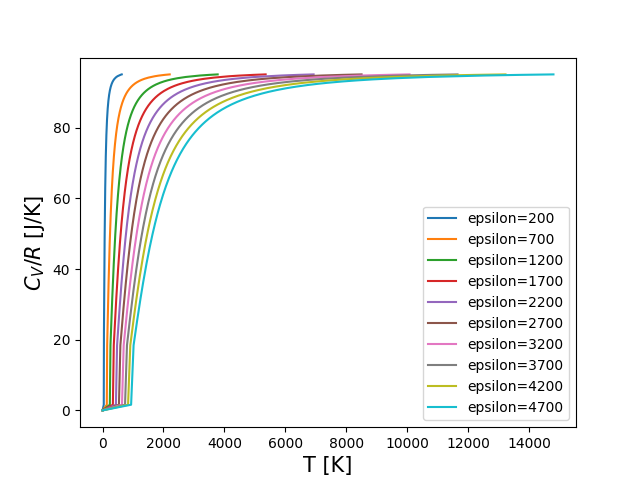
\includegraphics[width=8cm]{../figures/C_comparrison.png}
\caption{Heat capacity $C_V$ for different $\epsilon$.}
\label{fig:comparrison}
\end{figure}

\section*{Appendix III.}
Since we have that 
$$U=NkT=\epsilon q+\frac{N}{2}\epsilon$$ 
for the Einstein crystal, we can see that
$$ dU=NkdT=\epsilon dq\Leftrightarrow dT=\frac{\epsilon}{Nk}dq.$$
We can use this to model how $q$ changes in the mug, changes the temperature of the mug material. But the Einstein solid is not valid for liquids. The Temperfect mug has a material that will melt when you put hot liquid in the mug and therefore the Einstein model is not valid at that point. After a period of time the mug material will go back into solid and here the Einstein model might be valid. As energy units is transferred from the mug material to the liquid in the mug. 

\section*{Appendix CODES. Termos temperature}
This code plots the temperatures as a function of time for the two thermos cups.
\begin{lstlisting}
import matplotlib.pyplot as plt
import numpy as np
path_data = "../data_files/"

infile = open(path_data+"termokopper.txt","r")

kopp1 = []
kopp2 = []
t = []

for line in infile:
    line = line.split()
    t.append(eval(line[0]))
    kopp1.append(eval(line[1]))
    kopp2.append(eval(line[2]))
infile.close()

t = np.asarray(t)
kopp1 = np.asarray(kopp1)
kopp2 = np.asarray(kopp2)*1.12



plt.plot(t,kopp1,label="Bodum mug")
plt.plot(t,kopp2,label="Temperfect mug")
plt.xlabel("t $[s]$",FontSize=15)
plt.ylabel(r"T $[^{\circ}C]$",FontSize=15)
plt.legend()
plt.savefig("../figures/mugs.png")
plt.clf()

plt.plot(t,kopp1,label="Bodum mug")
plt.plot(t,kopp2,label="Temperfect mug")
plt.xlabel("t $[s]$",FontSize=15)
plt.ylabel(r"T $[^{\circ}C]$",FontSize=15)
plt.xlim(0,150)
plt.ylim(85,90)
plt.legend()
plt.savefig("../figures/mugs_2.png")
plt.clf()
\end{lstlisting}



\section*{Appendix CODES. Entropy H2O}
This code plots the entropy and heat capacity of H2O.
\begin{lstlisting}
import numpy as np
import matplotlib.pyplot as plt

def C(T):
    if T<=273.15:
        return 2.03 * 1e3
    elif T>=373.15:
        return 1.998 * 1e3
    else:
        return 4.184 * 1e3

N = int(1e4)
T = np.linspace(100,500,N)
dSdT = np.zeros(N)
for i in range(N):
    dSdT[i] = C(T[i])/T[i]

S = np.zeros(N)
sum = 0

dT = (T[-1]-T[0])/N
for i in range(N):
    S[i] = sum
    sum += C(T[i])/T[i]*dT

plt.plot(T,S)
plt.xlabel(r"T $[K]$",FontSize=15)
plt.ylabel(r"S $[J/K]$",FontSize=15)
plt.savefig("../figures/S_mot_T")
plt.clf()


plt.plot(T,dSdT)
plt.xlabel(r"T [$K$]",FontSize=15)
plt.ylabel(r"dS/dT [$J/K^2$]",FontSize=15)
plt.savefig("../figures/dSdT_mot_T")
plt.clf()
\end{lstlisting}
\section*{Appendix CODES. Entropy plotter}
This code plots the entropy as a function of S.
\begin{lstlisting}
import numpy as np
import matplotlib.pyplot as plt
from scipy.constants import k
from math import factorial

k = 1

N = int(300)
N_len = 800
q = np.linspace(1,N_len,N_len)
dq = (q[-1]-q[0])/(len(q)-1)


omega = np.zeros(N_len)
for i in range(0,N_len):
    omega[i] = factorial(int(q[i])+N-1)/(factorial(int(q[i]))*factorial(N-1))
S = k*np.log(omega)

dqdS = np.zeros(N_len)

for i in range(1,N_len):
    dqdS[i] = dq/(S[i]-S[i-1])
T = dqdS

Cv = np.zeros(N_len)
for i in range(1,N_len):
    Cv[i] = dq/(T[i]-T[i-1])


plt.plot(q,Cv/N,label=r"$N=%g$"%(N_len))
plt.xlabel("q",FontSize=15)
plt.ylabel(r"$C_V/Nk$",FontSize=15)
plt.legend()
plt.savefig("../figures/C_mot_q.png")
plt.clf()

plt.plot(q,S,label=r"$N=%g$"%(N_len))
plt.xlabel("q",FontSize=15)
plt.ylabel(r"$S/k$",FontSize=15)
plt.legend()
plt.savefig("../figures/S_mot_q.png")
plt.clf()

outfile = open("../data_files/numerical_data.txt","w+")
outfile.write("q Omega S T Cv/Nk N=%g\n"%(N_len))
for i in range(N_len):
    outfile.write("%g %.5f %.5f %.5f %.5f\n"%(q[i],omega[i],S[i],T[i],Cv[i]/N))
outfile.close()
\end{lstlisting}
\section*{Appendix CODES. $\Omega$ comparrison.}
This code plots the high T vs low T vs Stirling approx. for the Omegas.
\begin{lstlisting}
import numpy as np
import matplotlib.pyplot as plt

N = 1e2
N_len = int(1e3)

q = np.linspace(1,N_len,N_len)
omega_lowT = (N*np.exp(1)/q)**q
omega_highT = (q*np.exp(1)/N)**N
omega_stirling = ((q+N)/q)**q * ((q+N)/N)**N

plt.plot(q,np.log(omega_lowT),label=r"$\Omega_{low\ T}$, N=%g"%(N))
plt.plot(q,np.log(omega_highT),label=r"$\Omega_{high\ T}$, N=%g"%(N))
plt.plot(q,np.log(omega_stirling),label=r"$\Omega_{Stirling}$, N=%g"%(N))
plt.xlabel("q",FontSize=15)
plt.ylabel("S/k",FontSize=15)
plt.legend()
plt.savefig("../figures/omegas.png")
plt.clf()
\end{lstlisting}
\section*{Appendix CODES. Analytical vs Numerical entropy}
This code plots the analytical vs the numerical entropy.
\begin{lstlisting}
import numpy as np
import matplotlib.pyplot as plt

k = 1;

infile = open("../data_files/numerical_data.txt","r")
N = infile.readline().split("=")[-1]
N = eval(N)

q = []
omega_numerical = []
S_numerical = []
T_numerical = []
Cv_over_Nk_numerical = []

for line in infile:
    line = line.split()
    q.append(eval(line[0]))
    omega_numerical.append(eval(line[1]))
    S_numerical.append(eval(line[2]))
    T_numerical.append(eval(line[3]))
    Cv_over_Nk_numerical.append(eval(line[4]))
infile.close()
q = np.asarray(q)
omega_numerical = np.asarray(omega_numerical)
S_numerical = np.asarray(S_numerical)
T_numerical= np.asarray(T_numerical)
Cv_over_Nk_numerical= np.asarray(Cv_over_Nk_numerical)


S_analytical = N*k*np.log(2*q/N+1)
plt.plot(q,S_analytical)
plt.plot(q,S_numerical)
plt.show()
\end{lstlisting}

\section*{Appendix CODES. $C$ comparrison.}
This code plots the different $\epsilon$'s.
\begin{lstlisting}
import numpy as np
import matplotlib.pyplot as plt
from scipy.constants import k
from scipy.constants import R


k = 1;

infile = open("../data_files/numerical_data.txt","r")
N = infile.readline().split("=")[-1]
N = eval(N)

q = []
omega_numerical = []
S_numerical = []
T_numerical = []
Cv_over_Nk_numerical = []

for line in infile:
    line = line.split()
    q.append(eval(line[0]))
    omega_numerical.append(eval(line[1]))
    S_numerical.append(eval(line[2]))
    T_numerical.append(eval(line[3]))
    Cv_over_Nk_numerical.append(eval(line[4]))
infile.close()
q = np.asarray(q)
omega_numerical = np.asarray(omega_numerical)
S_numerical = np.asarray(S_numerical)
T_numerical= np.asarray(T_numerical)
Cv_over_Nk_numerical= np.asarray(Cv_over_Nk_numerical)

plt.yticks()
for epsilon in range(200,5001,500):
    plt.plot(T_numerical*epsilon,Cv_over_Nk_numerical*N*k/R,label="epsilon=%g"%(epsilon))
plt.xlabel("T [K]",FontSize=15)
plt.legend()
plt.savefig("../figures/C_comparrison.png")
plt.clf()
\end{lstlisting}


%% all \section commands following \appendix are automatically taken as appendices

%% Note that \label{appendix} command on line 115. What this does is setup a reference point for LaTeX that you can
%% access wherever you want using \ref{appendix}.
%% You can place labels on most environments such as equations, figures, tables, etc.


%% If you want to include figure:
%\includegraphics[scale=1.0]{filename}
%% check https://en.wikibooks.org/wiki/LaTeX/Importing_Graphics if you want to know more

\end{document}
